The construction of the Alam robot platform was successfully completed using steel rod segments, as depicted in Figure \ref{fig:arm-segments}. The constraints are securely fastened to the rods, thereby ensuring stability and structural integrity.

\begin{figure}[H]
    \centering
    \includegraphics[width=0.6\textwidth]{arm-segments}
    \caption{Arm segments}
    \label{fig:arm-segments}
\end{figure}

Figure \ref{fig:arm-positions} illustrates the robot in three different poses using a single segment. The first pose shows the arm to the left, the second a straight configuration, and the third with the arm to the right. The actuators exhibited sufficient friction and force to maintain each position effectively.

\begin{figure}[H]
    \centering
    \begin{subfigure}[b]{0.3\textwidth}
        \includegraphics[width=\textwidth]{arm-left}
        \caption{Arm to the left}
        \label{fig:arm-left}
    \end{subfigure}
    \begin{subfigure}[b]{0.3\textwidth}
        \includegraphics[width=\textwidth]{arm-straight}
        \caption{Straight arm}
        \label{fig:arm-straight}
    \end{subfigure}
    \begin{subfigure}[b]{0.3\textwidth}
        \includegraphics[width=\textwidth]{arm-right}
        \caption{Arm to the right}
        \label{fig:arm-right}
    \end{subfigure}
    \caption{One segment arm positions}
    \label{fig:arm-positions}
\end{figure}

The firmware and control application demonstrated satisfactory functionality during testing. However, the firmware remains incomplete, particularly with regard to its ability to handle commands with erroneous parameters. The majority of the code functionalities were tested, but certain aspects related to the EEPROM memory and robot status display were not yet fully implemented. Furthermore, the functionality of the joystick control remains unimplemented.

\begin{figure}[H]
    \centering
    \includegraphics[width=0.6\textwidth]{electronics}
    \caption{Electronics case and connections}
    \label{fig:electronics}
\end{figure}


The electronics case, shown in Figure \ref{fig:electronics}, was initially prototypical, utilizing a breadboard and jumper wires for connections. This configuration was found to cumbersome and prone to disconnection, which made the assembly and debugging processes more complex.

Figure \ref{fig:complete-prototype} compares the prototype with two segments against the initial design. The prototype closely resembles the design, thereby demonstrating the successful realization of the intended structure.

\begin{figure}[H]
    \centering
    \begin{subfigure}[b]{0.3\textwidth}
        \includegraphics[width=\textwidth]{real-model}
        \caption{Real prototype}
        \label{fig:real-model}
    \end{subfigure}
    \begin{subfigure}[b]{0.3\textwidth}
        \includegraphics[width=\textwidth]{design-model}
        \caption{Designed prototype}
        \label{fig:design-model}
    \end{subfigure}
    \caption{Complete prototype}
    \label{fig:complete-prototype}
\end{figure}

Issues encountered with the linear actuators are shown in Figure \ref{fig:manufacturing-issues}. These include discrepancies in tolerance, alignment challenges between rod and bearing, printing errors, and base deformation due to spring force, which has occasionally resulted in detachment of the arm from its support.

\begin{figure}[H]
    \centering
    \begin{subfigure}[t]{0.6\textwidth}
        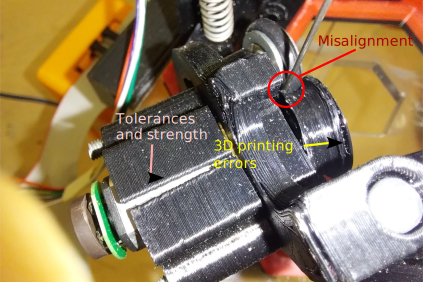
\includegraphics[width=\textwidth]{fdm-issues}
        \caption{Fabrication and alignment}
        \label{fig:fdm-issues}
    \end{subfigure}
    \begin{subfigure}[t]{0.3\textwidth}
        \includegraphics[width=\textwidth]{arm-spring-issue}
        \caption{Spring and arm}
        \label{fig:arm-spring-issue}
    \end{subfigure}
    \caption{Linear actuator issues}
    \label{fig:manufacturing-issues}
\end{figure}


Finally, Table \ref{tab:platform-specifications} presents general specifications of the platform, including height, maximum arm reach, body dimensions, and actuator tolerances.

\begin{table}[h]
    \centering
    \caption{Platform specifications}
    \label{tab:platform-specifications}
    \begin{tabular}{ll}
    \toprule
    Property & Value \\
    \midrule
    Height  & 30 cm \\
    Maximum height (with arm) & 70 cm \\
    Weight & 1 kg \\
    Linear actuators tolerance & $\pm$1 mm \\
    \bottomrule
    \end{tabular}
\end{table}